\documentclass[onecolumn, draftclsnofoot,10pt, compsoc]{IEEEtran}
\usepackage[utf8]{inputenc}
\usepackage{lscape}
\usepackage{pgfgantt}
\usepackage{graphicx}
\usepackage{setspace}
\usepackage{url}
\usepackage{import}
\usepackage{pdfpages}
\usepackage{caption}
\usepackage{geometry}
\usepackage{listings}
\usepackage{color}

\definecolor{codegreen}{rgb}{0,0.6,0}
\definecolor{codegray}{rgb}{0.5,0.5,0.5}
\definecolor{codepurple}{rgb}{0.58,0,0.82}
\definecolor{backcolour}{rgb}{0.95,0.95,0.92}

\lstdefinestyle{mystyle}{
	backgroundcolor=\color{backcolour},   
	commentstyle=\color{codegreen},
	keywordstyle=\color{magenta},
	numberstyle=\tiny\color{codegray},
	stringstyle=\color{codepurple},
	basicstyle=\footnotesize,
	breakatwhitespace=false,         
	breaklines=true,                 
	captionpos=b,                    
	keepspaces=true,                 
	numbers=left,                    
	numbersep=5pt,                  
	showspaces=false,                
	showstringspaces=false,
	showtabs=false,                  
	tabsize=2
}

\lstset{style=mystyle}
\geometry{textheight=9.5in, textwidth=7in}

\def \CapstoneTeamName{		Ebola Team}
\def \CapstoneTeamNumber{		34}
\def \GroupMemberOne{			Claude Maimon}
\def \GroupMemberTwo{			Brian Lee Huang}
\def \GroupMemberThree{			Bianca Beauchamp}
\def \CapstoneProjectName{		Ebola Prediction Model}
\def \CapstoneSponsorCompany{	Professor Bill Smart}


\def \DocType{		Final Report
	%Requirements Document
	%Technology Review
	%Design Document
	%Progress Report
}

\newcommand{\NameSigPair}[1]{\par
	\makebox[2.75in][r]{#1} \hfil 	\makebox[3.25in]{\makebox[2.25in]{\hrulefill} \hfill		\makebox[.75in]{\hrulefill}}
	\par\vspace{-12pt} \textit{\tiny\noindent
		\makebox[2.75in]{} \hfil		\makebox[3.25in]{\makebox[2.25in][r]{Signature} \hfill	\makebox[.75in][r]{Date}}}}
% 3. If the document is not to be signed, uncomment the RENEWcommand below
\renewcommand{\NameSigPair}[1]{#1}

%%%%%%%%%%%%%%%%%%%%%%%%%%%%%%%%%%%%%%%
\begin{document}
	\begin{titlepage}
		\pagenumbering{gobble}
		\begin{singlespace}
			%\includegraphics[height=4cm]{coe_v_spot1}
			\hfill 
			% 4. If you have a logo, use this includegraphics command to put it on the coversheet.
			%\includegraphics[height=4cm]{CompanyLogo}   
			\par\vspace{.2in}
			\centering
			\scshape{
				\huge CS Capstone \DocType \par
				{\large\today}\par
				\vspace{.5in}
				\textbf{\Huge\CapstoneProjectName}\par
				\vfill
				{\large Prepared for}\par
				\Huge \CapstoneSponsorCompany\par
				\vspace{5pt}
				{\large Prepared by }\par
				Group\CapstoneTeamNumber\par
				% 5. comment out the line below this one if you do not wish to name your team
				\CapstoneTeamName\par 
				\vspace{5pt}
				{\Large
					\NameSigPair{\GroupMemberOne}\par
					\NameSigPair{\GroupMemberTwo}\par
					\NameSigPair{\GroupMemberThree}\par
				}
				\vspace{20pt}
			}
			\begin{abstract}
				There are four major parts to this project, image processing, machine learning, production and evaluation. The image processing portion will import the thermal images from the camera, format the images, select necessary pixels, and summarize those pixels into a single temperature value. The machine learning portion of the project will create a mathematical model to represent the relationship between skin temperature and core body temperature and then test this model on different sets of data. The production portion will use the model that has been created to produce a estimated core body temperature from the estimated skin temperature and then produce a true or false output as to weather or not thatThere are four major parts to this project, image processing, machine learning, production and evaluation. The image processing portion will import the thermal images from the camera, format the images, select necessary pixels, and summarize those pixels into a single temperature value. The machine learning portion of the project will create a mathematical model to represent the relationship between skin temperature and core body temperature and then test this model on different sets of data. The production portion will use the model that has been created to produce a estimated core body temperature from the estimated skin temperature and then produce a true or false output as to weather or not that
				
			\end{abstract}  
		   
		\end{singlespace}
	\end{titlepage}
	\newpage
	\pagenumbering{arabic}
	\tableofcontents
	% 7. uncomment this (if applicable). Consider adding a page break.
	%\listoffigures
	%\listoftables
	\clearpage
	
	\section{Introduction}
	
	There are four major parts to this project, image processing, machine learning, production and evaluation. The image processing portion will import the thermal images from the camera, format the images, select necessary pixels, and summarize those pixels into a single temperature value. The machine learning portion of the project will create a mathematical model to represent the relationship between skin temperature and core body temperature and then test this model on different sets of data. The production portion will use the model that has been created to produce a estimated core body temperature from the estimated skin temperature and then produce a true or false output as to weather or not that subject has a fever. The evaluation portion will evaluate how accurate the true or false output of the production portion is. The machine learning, production and evaluation portions will have user interfaces. The first piece of the project that will be developed is be the image processing portion since both the learning, and production code rely on processing the thermal image to get a skin temperature. The second piece that will be worked on is the machine learning portion since the model needs to be created and tested before it goes into production. The third piece that will be done is the production portion and the forth piece that will be done is the evaluation portion.
	
	Who requested it?
	
	Why was it requested?
	
	What is its importance?
	
	Who was/were your client(s)?
	
	Who are the members of your team?
	
	What were their roles?
	
	What was the role of the client(s)? \(I.e., did they supervise only, or did 
	they participate in doing development\)
	
	
	\section{Requirements Document}
	\subsection{Old Requirement Document}
	\import{sections/}{requirments.tex}
	\subsection{New Requirements}
	There were two main things that we changed in the requirement documents. The first was the 40\% success rate. From the initial research that we did, we found that some previous attempts of this approach produced about 40\% success rate. When we started the project we thought that we could achieve that success rate. However, as we'll discuss in this report, we ran into many problems with the camera. The camera wasn't calibrated right and it returned bad values. We tried many things to fix it even though it is not in our requirements to try and fix the camera. When first writing this document, we assumed the camera would be working correctly. Since that wasn't the case, we had a hard time collecting good data. That's why we took out the 40\% success rate goal. Our client, Bill Smart, agreed with this change. Another change that we made was producing a report and not a research paper as a final product with the code. Our client agreed that there is no need for a research paper. We just needed to produce a report that will help his graduate students in continuing this project. 
	\subsection{Final Gantt Chart}
	\begin{center}
		\begin{landscape}
			\begin{ganttchart}[
				vgrid,
				x unit=0.75cm,
				y unit chart=1cm,
				hgrid style/.style=red
				]{24}{24}
				\gantttitle{Ebola Virus Project Process}{24} \\
				\ganttbar{Processing thermal image}{1}{5} \\
				\ganttbar{Process data from pixels}{5}{12} \\
				\ganttbar{Collecting Data}{12}{18} \\
				\ganttbar{Analyzing data}{18}{20} \\
				\ganttbar{Mathematical model}{11}{17} \\
				\ganttbar{Testing and result analyzing}{18}{19} \\
				\\[grid]
				\ganttbar{Program for graduate students}{15}{17} \\
				\ganttbar{Testing and result analyzing}{18}{19} \\
				
				\ganttbar{Stretch goals}{19}{20} \\
				\ganttlink{elem0}{elem1}
				\ganttlink{elem1}{elem3}
				\ganttlink{elem2}{elem3}
				\ganttlink{elem3}{elem4}
				\ganttlink{elem4}{elem5}
				\ganttlink{elem5}{elem6}
				\ganttlink{elem6}{elem7}
			\end{ganttchart}
		\end{landscape}
	\end{center}
	
	\section{Design Document}
	\subsection{Original Design Document}
	\import{sections/}{Design_Document.tex}
	\subsection{New Design Changes}
	add changes	
	
	\section{Tech Reviews}
	\subsection{Brian's Tech Review}
	\import{sections/}{Brian_Huang_Tech_Review.tex}
	\subsection{Claude's Tech Review}
	\import{sections/}{Claude_tech.tex}
	\subsection{Bianca's Tech Review}
	\import{sections/}{Binaca_tech.tex}
	
	\section{Weekly Blog Posts}
	
	\subsection{Brian}
	\import{sections/}{Brian_weekly.tex}
	
	\subsection{Claude}
	\import{sections/}{Claude_weekly.tex}
	
	\subsection{Bianca}
	\import{sections/}{Bianca_weekly.tex}
	\newpage
	\section{Final Poster}	
		Our final poster as it was presented at the undergraduate engineeting expo. 	
		\begin{figure}[!hb]
			\centering
			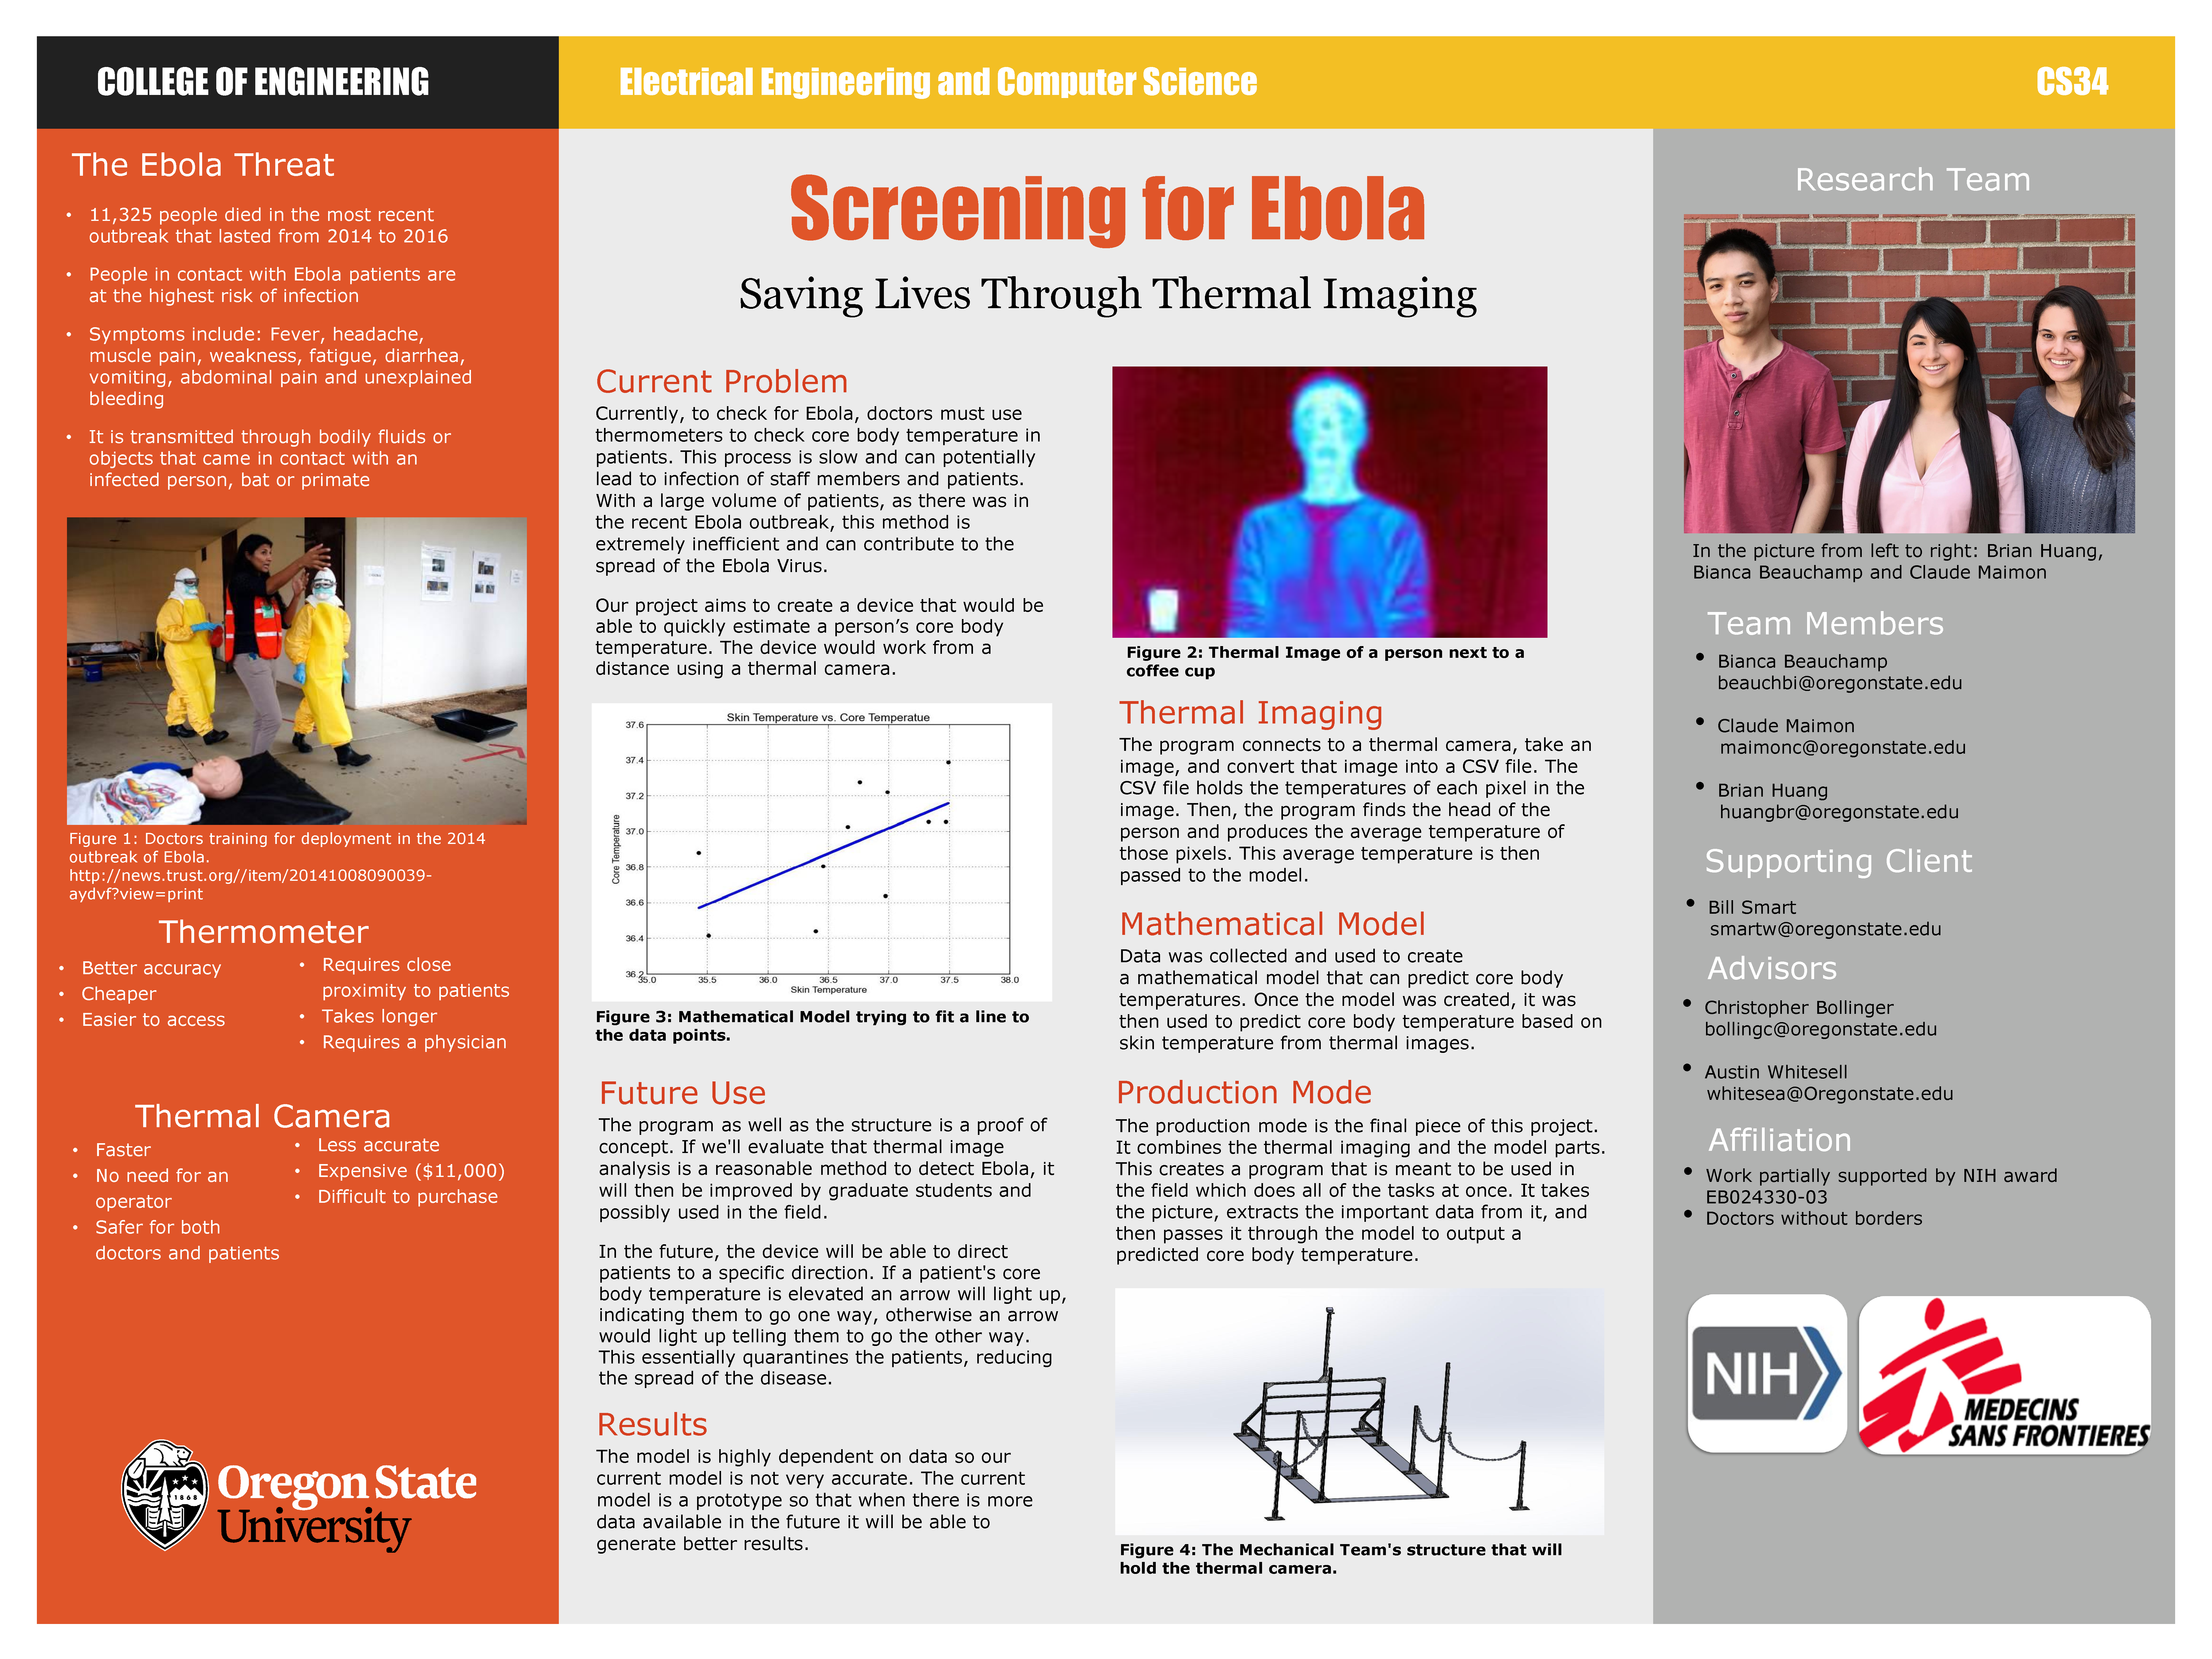
\includegraphics[width=\textwidth,  height=20cm]{Group34NewPost.eps}
			\caption{Our final poster}
		\end{figure}

	\section{Project Documentation}
	\import{sections/}{documentation.tex}
	
	\section{Recommended Technical Resources}
	
	\section{Conclusions and Reflections}
	\section{Appendix 1: Essential Code Listings}
	%	\import{sections/}{Appendix_1.tex}
	\section{Appendix 2}
	
	
	\bibliographystyle{IEEEtran}
	\bibliography{mybib}
	
\end{document}
